% !TEX TS-program = pdflatexmk
\documentclass[12pt]{article}

% Layout.
\usepackage[top=1in, bottom=0.75in, left=1in, right=1in, headheight=1in, headsep=6pt]{geometry}

% Fonts.
\usepackage{mathptmx}
\usepackage[scaled=0.86]{helvet}
\renewcommand{\emph}[1]{\textsf{\textbf{#1}}}
\newcommand{\ans}[1][1in]{\rule{#1}{.5pt}}

\usepackage[parfill]{parskip}

% Misc packages.
\usepackage{amsmath,amssymb,latexsym}
\usepackage{graphicx,hyperref}
\usepackage{array}
\usepackage{xcolor}
\usepackage{multicol,tikz}
\usepackage{tabularx,colortbl,booktabs,xparse}
\usepackage{enumitem}

% Rotation: \rot[<angle>][<width>]{<stuff>}
\NewDocumentCommand{\rot}{O{45} O{1em} m}{\makebox[#2][l]{\rotatebox{#1}{#3}}}%

\usepackage{fancyhdr}
\pagestyle{fancy} 
\lhead{\large\sf\textbf{MATH F113X: Dijkstra's Algorithm}}
%\chead{\large\sf\textbf{lecture notes}}
%\rhead{\large\sf\textbf{Day 1}}

\begin{document}



\vfill

\begin{center} Air North Route Map \end{center}

\begin{center} \includegraphics[width = .8\textwidth]{AirNorthRouteMap.jpg} \end{center}

\vfill
\begin{center} Alaska and Hawaii Airlines Combined Route Math \end{center}
\begin{center} \includegraphics[width = .8\textwidth]{CombinedRouteMap.jpg}\end{center}

\vfill

\newpage
\fbox{Dijkstra's Algorithm}

\textbf{input:} a graph with distances (weights) on the edges, a starting vertex, say $s$ and end ending vertex, say $e$\\
\textbf{output:} the length of the shortest path between $s$ and $e$\\
\textbf{rough strategy:} Starting with the ending vertex, work your way back to the starting vertex keeping track of the shortest path \textbf{thus far.}\\
\textbf{Steps:}
\begin{enumerate}
	\item  Mark the ending vertex with a distance of zero and label it as \emph{current}.
	\item  Let $v$ be the current vertex. For every vertex $w$ with an edge to $v$ \emph{that has not already been visited}, calculated the distance to $e$ through $v$ and mark $w$ with this distance \emph{unless its present distance is smaller.}** (This is called the tentative distance to $e$.)
	\item Mark the current vertex as visited. We never look at this vertex again.
	\item Identify the \emph{un-visited} vertex with the smallest distance to $e$. Mark it as current and return to step 2. You know when to stop when vertex $s$ is labeled as current.
\end{enumerate}
** If you keep track of which current vertex assigns a minimum distance, you can recover the shortest path itself, not just the length.\\	
			
\hrule

\vspace{1cm}

\begin{minipage}{.4\linewidth}
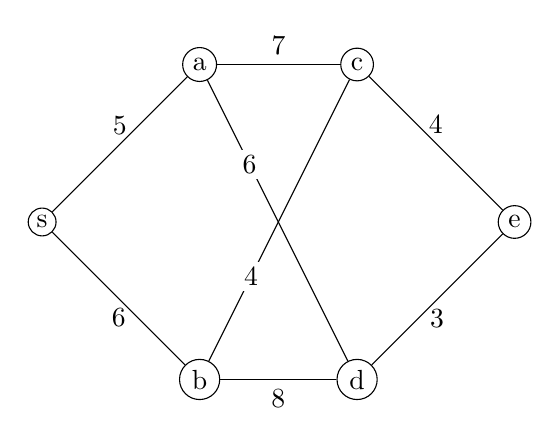
\begin{tikzpicture}[scale=2]
\node[draw,circle, inner sep=1.5pt](s) at (0,0){s};
\node[draw,circle, inner sep=2pt](a) at (1,1){a};
\node[draw,circle, inner sep=2pt](b) at (1,-1){b};
\node[draw,circle, inner sep=2pt](c) at (2,1){c};
\node[draw,circle, inner sep=2pt](d) at (2,-1){d};
\node[draw,circle, inner sep=2pt](e) at (3,0){e};
\draw (s) -- (a) node [midway,above]{5};
\draw (s) -- (b) node [midway,below]{6};
\draw (a) -- (c) node [midway,above]{7};
\draw (a) -- (d) node [pos = .3, inner sep = 2pt, fill = white]{6};
\draw (b) -- (c) node [pos = .3, inner sep = 2pt, fill = white]{4};
\draw (b) -- (d) node [midway,below]{8};
\draw (d) -- (e) node [midway,below]{3};
\draw (c) -- (e) node [midway,above]{4};
\end{tikzpicture}
\end{minipage}
%%%%%%%
% 
 \hspace{1cm}
%
  \begin{minipage}[t]{.6\linewidth}
 \begin{tabular}{ |c | c |c| c|}
 \hline
 &&\textbf{tentative}&\\
 vertex & current/ & minimum& preceding\\ 
 &visited&\quad distance to $e$ \quad& vertex\\
 \hline
s&&& \\
\hline 
a&&& \\
\hline 
b&&& \\
\hline 
c&&& \\
\hline 
d&&& \\
\hline 
e&&& \\
\hline 
 \end{tabular}
  \end{minipage}
  
  \bigskip

Length of the shortest path from $s$ to $e$: \underline{\hspace{1in}}\\

Find the shortest path from $s$ to $e$ \emph{using the last column in the table.}
\vfill


\vfill
Think of another application of Dijkstra's Algorithm. It must include: vertices, weights of edges, and the meaning of a shortest path.

\vfill
\bigskip
\end{document}